\chapter{Introducción}

% =============================================================================
% ¿Qué se hizo?
% =============================================================================
En este trabajo se obtuvo un diseño preliminar de la geometría de los  sistemas
de intercambio de gases del MRCVC \cite{toth}, con el objetivo de maximizar el
rendimiento volumétrico del motor en un rango de velocidades.
%
La optimización se realizó utilizando en conjunto una serie de herramientas de
simulación, de las cuales las principales fueron: 

\begin{itemize}
        %
    \item ICESym \cite{icesym}, simulador de motores de combustión interna.
        %
    \item OpenFOAM \cite{openfoam}, la herramienta libre de CFD.
        %
    \item Salome \cite{salome}, plataforma libre para simulación númerica.
        %
\end{itemize}


Además, se desarrolló un sencillo optimizador capaz de generar y evaluar
diferentes geometrías con el fin de buscar una combinación de parámetros que
maximicen el rendimiento volumétrico del motor para un rango de velocidades
determinado.

% Además, se desarrolló una serie de herramientas sencillas para: configurar,
% ejecutar y evaluar resultados del simulador ICESym; PRE y POST procesar las
% corridas de OpenFOAM.

El proceso de optimziación consta de una primer aproximación utilizando
coeficientes de descarga ($C_{D}$) estimados en trabajos anteriores
\cite{lopez13}, con los cuales se evaluó el funcionamiento del los parámetros
que definen la geometría de los sistemas de intercambio de gases, en
particular: diámetros, longitudes y reglaje o posición angular de los mismos.
%NOTA: nunca dije que es un cd y por que importa, pero tampoco se como ponerlo

Utilizando el algoritmo genético se evaluó una gran cantidad de geometrías,
dando puntaje a cada una luego de simular el ciclo operativo del motor con
ICESym y puntuar las curvas de rendimiento volumétrico obtenidas con una
función objetivo.

El diseño preliminar se volcó en un modelo de CAD de los puertos con los cuales
se realizó una serie de flujometrías, evaluando el coeficiente de descarga
($C_D$) de ambos puertos en diferentes posiciones del conjunto rotante, con el
fin de obtener un mapa del $C_D$ en función de dos variables: \emph{alzada}
equivalente y diferencia de presión.
%
Este mapa de $C_{D}$ se utilizó como retroalimentación del simulador ICESym
para repetir los pasos descritos anteriormente y así obtener un diseño
satisfactorio.

% =============================================================================
% ¿Por qué se hizo?
% =============================================================================
La motivación de este trabajo surge del deseo de continuar con el desarrollo
del MRCVC, en particular mejorar el pre diseño de los sistemas de intercambio
de gases, sentando la base para una futura optimización de los mismos en un
motor con requisitos de diseño concretos.

\section{MRCVC}
%
El MRCVC es un proyecto que surgió en la Universidad Nacional del Comahue,
inventado y patentado por Jorge Toth\cite{toth} en el año 2004, este proyecto
nace en el marco del \emph{Proyecto de Investigación Desarrollo de modelos y
herramientas para la simulación de problemas complejos en ingeniería mediante
fluido dinámica computacional (04/I-251)}. Actualmente se encuentra en etapa de
desarrollo.

\begin{figure}
    \centering
    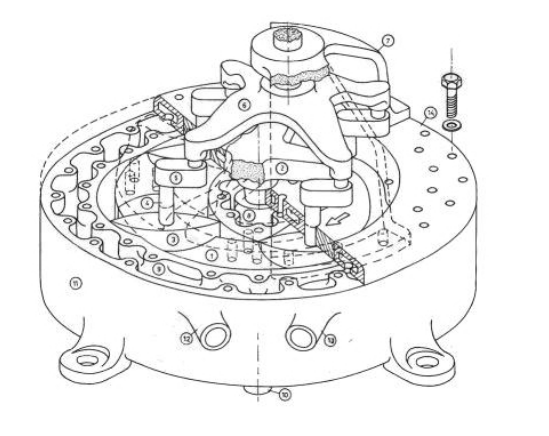
\includegraphics[width=0.5\textwidth]{perspectiva_mrcvc.png}
    \caption{Motor Rotativo de Combustión a Volumen Constante}
    \label{fig:mrcvc}
\end{figure}

En trabajos anteriores\cite{lopez16, lopez13, roldan} se han mencionado las
características que hacen al MRCVC un motor atractivo, la geometría de la
cámara de combustión y del conjunto rotante permiten  combustión a volumen
constante y un balanceo mecánico de fuerzas.
%
Esto permite un funcionamiento más suave del motor, además de una reducción del
ruido y desgaste en comparación a motores rotativos tradicionales (Wankel) y
alternativos.
%
No obstante a esto hay que mencionar que los motores rotativos traen consigo
una serie de problemas como la necesidad de introducir aceite a la cámara de
combustión para lubricar elementos móviles, el solape de cámaras durante la
apertura de los puertos y en particular al MRCVC un complejo sistema de
sellos\cite{roldan}.


\section{Sistema de Intercambio de Gases}
%
El sistema de intercambio de gases es el objeto de este trabjo, se ocupa de los
procesos de admisión y escape que consistenen admitir una carga de mezcla
fresca y expulsar los gases quemados al final de cada ciclo.
%
La masa de aire inductada limita la cantidad de combustible que se puede
quemar, del mismo modo que la cantidad de gases quemados que se pueden extraer
al final de cada ciclo, limita la cantidad de masa fresca que puede ingresar a
la cámara de combustión.
%
Por estos motivos es importante que la geometría de este sistema permita que
estos procesos se realicen de manera eficiente, maximizando la cantidad de mezcla
disponible para la combustión en cada ciclo.
%
Otros objetivos del sistema de intercambio de gases son el de preparar la
mezcla\footnote{En el caso de motores SI que admiten mezclas de aire y
combustible} y brindar un flujo que favorezca el proceso de combustión.



El MRCVC no posee válvulas que indiquen el inicio y fin de los procesos
de adisión y escape, sino que posee puertos de admisión y escape similares a
lumbreras.
%
Esto significa que sin un mecanismo adicional, la posición y geometría de los
mismos define el inicio y fin de los procesos de admisión.

En la figura \ref{fig:valvulas} se observa un corte transversal de un puerto de
admisión de un motor con válvulas y en la figura \ref{fig:puertos} las
lumbreras de admisión y escape de un motor Wankel.

\begin{figure} \centering
    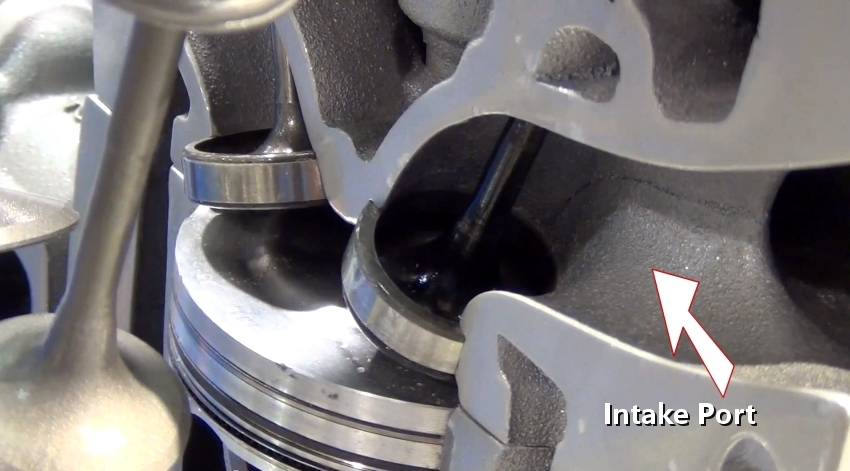
\includegraphics[width=0.5\textwidth]{ports_cut.png}
    \caption{Puerto de admisión en un motor con válvulas} 
    \label{fig:valvulas}
    % http://www.2carpros.com/images/articles/original/intake_port.jpg
\end{figure}

\begin{figure} \centering
    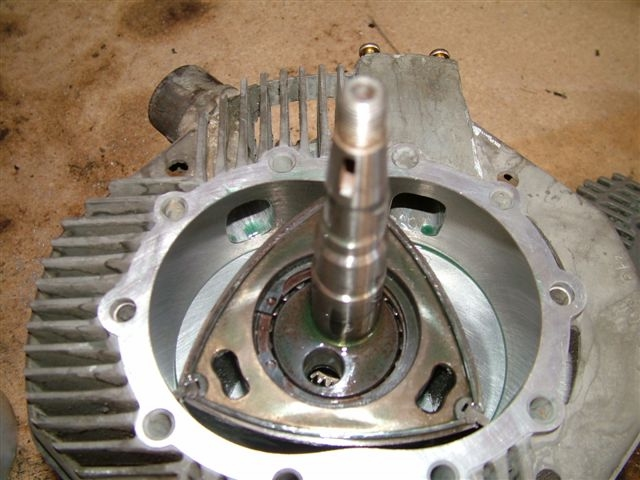
\includegraphics[width=0.5\textwidth]{puertos_rotativo.png}
    \caption{Puertos o lumbreras de admisión y escape} 
    \label{fig:puertos}
    % https://www.rx7club.com/attachments/old-school-other-rotary-63/290567d1207798173-latest-project-periphial-port-motorbike-km3-1.jpg
\end{figure}

Para la simulación del MRCVC se usa una sistema simplificado, que consta de un
tubo de diámetro $D$ y longitud $L$ tanto para la admisión como para el escape
(Fig. \ref{fig:sist_int_mrcvc}).
%
La apertura y cierre de los puertos es controlada por la posición angular de
los mismos en el estator.

% NOTA: aca podria poner una comparativa de rendimientos volumetricos, potencia y
% torque para un motor con puertos con mayor y menor apertura, mayor y menor
% diametro

\begin{figure}
    \centering
    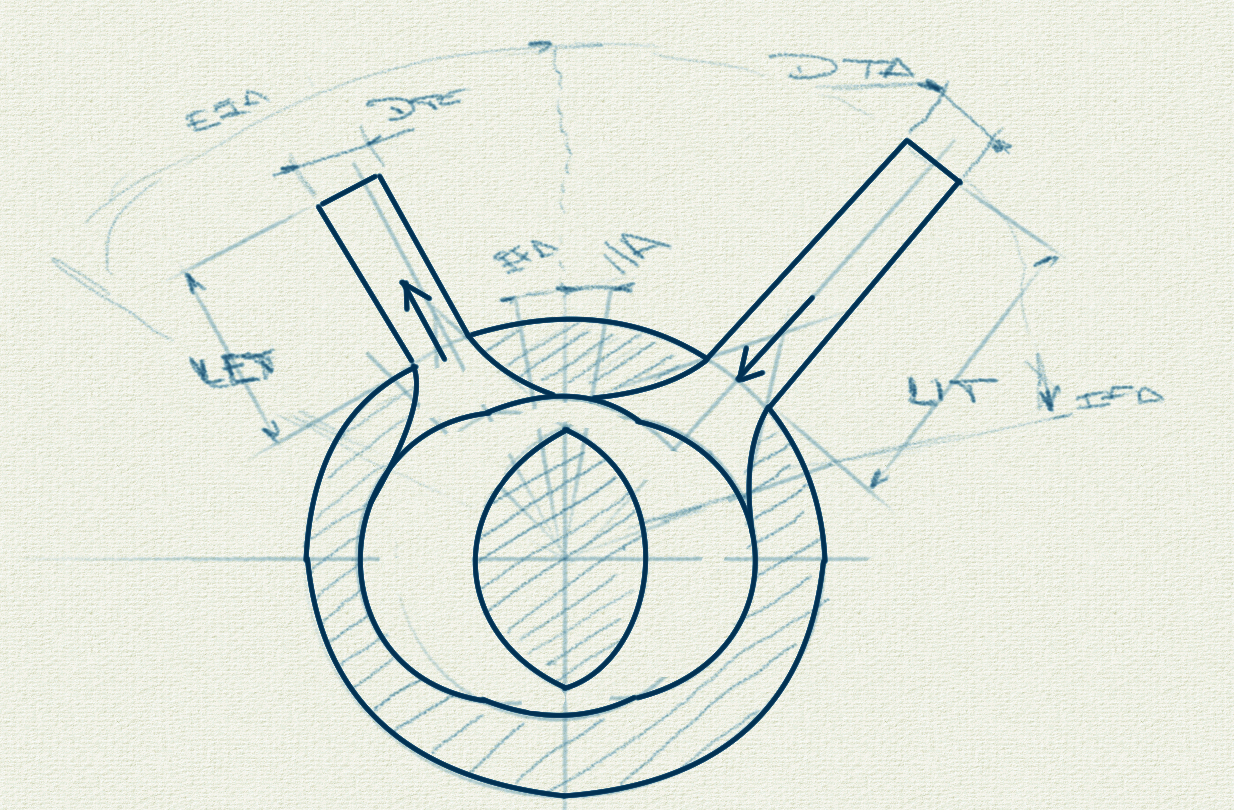
\includegraphics[width=0.5\textwidth]{croquis_motor.png}
    \caption{Parametros a modificar}
    \label{fig:croquis_mrcvc}
\end{figure}

En trabajos anteriores \cite{chiquito} se determinó que los puertos ubicados
sobre el cuerpo estatórico daban mejores resultados que los ubicados en la
"tapa" del motor.
% NOTA: tapa no es el término adecuado

\subsection{Indicadores de rendimiento}
\label{sec:indicadores_rendimiento}

Se medirá la eficiencia del sistema de intercambio de gases utilizando
exclusivamente el rendimiento volumétrico, $\eta_v$.
%
Es un parámetro comunmente utilizado para medir el rendimiento de motores
naturalmente aspirados.

% Los conductos de admisión restringen el flujo de aire hacia el motor, para
% medir la eficiencia con la que se está admitiendo aire al motor se define el
% rendimiento volumétrico $\eta_v$.
%
Se define como la relación entre el caudal volumétrico de aire que ingresa
al sistema de admisión y la velocidad a la que cambia el volumen dentro de un
cilindro.

\begin{equation}
  \label{eq:rendVol}
  \eta_v = \frac{2 \dot{m}_a}{\rho_{a,i} V_d N}
\end{equation}

Donde: $\rho_{a,i}$ es la densidad del aire a la entrada del sistema de
admisión (para motores naturalmente aspirados), también se puede definir
$\eta_v$ como:

\begin{equation}
    \label{eq:rendVol2}
    \eta_v = \frac{m_a}{\rho_{a,i} V_d}
\end{equation}

Dónde $m_a$ es la masa inductada al cilindro en cada ciclo.
%
Hay varios factores que afectan al rendimiento volumétrico, entre los más
importantes están:

\begin{enumerate}
    %
    \item Efectos cuasiestáticos
    %
    \item Pérdidas de carga por fricción viscosa
    %
    \item Pérdidas de carga en los puertos de admisión y escape
    %
    \item Transferencia de calor en sistema de admisión
    %
    \item Reglaje de los válvulas/puertos
    %
    \item Bloqueos de flujo en puertos de admisión y escape
    %
    \item Transferencia de calor en el cilindro
    %
    \item Sintonía del puerto de admisión y escape
    %
    \item Métodos de sobrecarga 
\end{enumerate}

Para este trabajo es de interés particular la pérdida de carga en los puertos,
el reglaje y la sintonía de admisión y escape.
%
En trabajos anteriores \cite{lopez13} se demostró que se tiene una mejor
\emph{performance} del motor si se ubican los puertos en el cuerpo central del
estator, realizando un optimización de la geometría mediante un barrido
paramétrico de las variables geométricas que determinan la forma, posición y
reglaje de los puertos.
%
% La ubicación angular de los puertos determina la duración de los procesos de
% admisión y escape, además de modificar la forma y el coeficiente de descarga.

Estos parámetros se ajustan o seleccionan teniendo en cuenta requisitos de
funcionamiento del motor, por lo que fue necesario establecer una curva de
rendimiento volumétrico para que la simulación numérica del
ciclo termodinámico se pueda acoplar al algoritmo de optimización y de este
modo evaluar los motores contra la curva de rendimiento requerida.
%
El criterio de diseño/selección de la curva de $\eta_v$ fué el siguiente:

\begin{itemize}
  \item que tenga un máximo de rendimiento entre 4000 y 6000 rpm.
  \item que la curva sea suave
\end{itemize}

\subsection{Estrategias de simulación de motores}
%
Se simulará el ciclo operativo del MRCVC con ICEsym, este simulador utiliza
modelos 0D para la combustión y 1D para el flujo de gases a través de los
conductos (fuera de la cámara de combustión).

Esta es una herramienta muy útil ya que permite evaluar la \emph{performance}
de un motor a un costo computacional bajo además, la manera en que se
implementó la entrada y salida de datos permite utilizar el simulador como una
``caja negra'' de modo que se pudo implementar en un \emph{script} como una
función a la que se le otorga como entrada un conjunto de parámetros y devuelve
los resultados de la simulación en un formato que permite la lectura y
evaluación de los mismos.
%
Esta característica del programa es la que permitió acoplarlo con un algoritmo
genético para realizar la optimización de la geometría.


Como se mencionó en el apartado \ref{sec:indicadores_rendimiento}, en trabajos
previos se realizó un pre diseño de los puertos de admisión y escape.
%
En dicho trabajo se determinó coeficientes de descarga constantes
% En dicho trabajo se utilizaron coeficientes de descarga estimados y
% constantes
para simular el flujo en los puertos de admisión y escape.
%
Con el objetivo de modelar con mayor precisión el flujo a través de los puertos
se realizó una modificación al código de ICESym que permite utilizar una
variable adicional para modelar al $C_D$, con lo que se puede representar la
dependencia con la apertura del puerto como la diferencia de presión
instantánea como $C_D = f(lv, \Delta P)$.
